\documentclass[10pt,a4paper]{article}

\usepackage{titlesec}
\usepackage[round]{natbib}
\usepackage{authblk}
\usepackage{fullpage}
\usepackage[space]{grffile}
\usepackage{graphicx}
\usepackage{textcomp}
\usepackage{deluxetable}
\usepackage{longtable}
\usepackage[utf8]{inputenc}
\usepackage[ngerman,english]{babel}
\usepackage{float}
\usepackage[margin=1in]{geometry}
\usepackage{parskip}


%\usepackage{setspace}
%\usepackage[section]{placeins}
%\usepackage{xcolor}
%\usepackage{breakcites}
%\usepackage{lineno}
%\usepackage{hyphenat}
%\usepackage{latexsym}
%\usepackage{tabulary}
%\usepackage{booktabs,array,multirow}
%\usepackage{amsfonts,amsmath,amssymb}


\renewcommand{\familydefault}{\sfdefault}


%\def\preprint{}


\PassOptionsToPackage{hyphens}{url}
\usepackage[colorlinks = true,
linkcolor = blue,
urlcolor = blue,
citecolor = blue,
anchorcolor = blue]{hyperref}
\usepackage{etoolbox}
\makeatletter
%\patchcmd\@combinedblfloats{\box\@outputbox}{\unvbox\@outputbox}{}{%
% \errmessage{\noexpand\@combinedblfloats could not be patched}%
%}%
\makeatother



\renewenvironment{abstract}
 {{\bfseries\noindent{\abstractname}\par\nobreak}\footnotesize}
 {\bigskip}


% You can conditionalize code for latexml or normal latex using this.
\newif\iflatexml\latexmlfalse
\providecommand{\tightlist}{\setlength{\itemsep}{0pt}\setlength{\parskip}{0pt}}%

\AtBeginDocument{\DeclareGraphicsExtensions{.pdf,.PDF,.eps,.EPS,.png,.PNG,.tif,.TIF,.jpg,.JPG,.jpeg,.JPEG}}



% Edit this header.tex file to include frontmatter definitions and global macros
\newcommand{\beginappendix}{%
	\setcounter{table}{0}
	\renewcommand{\thetable}{A\arabic{table}}%
	\setcounter{figure}{0}
	\renewcommand{\thefigure}{A\arabic{figure}}%
}

% Add here any LaTeX packages you would like to load in all document blocks


% Add here any LaTeX macros you would like to load in all document blocks
% \def\example{This is an example macro.}

% -----

\iflatexml
% Add here any LaTeXML-specific commands

% -----

\else
% Add here any export style-specific LaTeX commands. These will only be loaded upon document export. 
% \paperfield{Subject domain of my document}
% \keywords{keyword1, keyword2}
% \corraddress{Author One PhD, Department, Institution, City, State or Province, Postal Code, Country}
% \fundinginfo{Funder One, Funder One Department, Grant/Award Number: 123456.}
\fi


\begin{document}

\title{Why do we have so many different hydrological models? A review based on the case of Switzerland}


\author[1]{Pascal Horton*}
\author[1]{Bettina Schaefli}
\author[1]{Martina Kauzlaric}
\affil[1]{Institute of Geography \& Oeschger Centre for Climate Change Research, University of Bern, Bern, Switzerland (pascal.horton@giub.unibe.ch)}


\date{}


\ifdefined\preprint
\setcounter{page}{0}
\hrulefill

This manuscript has been submitted for publication in \textbf{WIREs Water}. Please note that it has not been peer-reviewed and has not yet been accepted for publication. Subsequent versions of this manuscript may have different content. If accepted, the final version of this manuscript will be available via the ‘Peer-reviewed Publication DOI' link on the right-hand side of this webpage. Please feel free to contact any of the authors; we welcome feedback

\hrulefill
\newpage
\fi

\begingroup
%\let\center\flushleft
%\let\endcenter\endflushleft
\maketitle
\endgroup




\begin{abstract}
Hydrology plays a central role in applied and fundamental environmental sciences, but it is well known to suffer from an overwhelming diversity of models, particularly to simulate streamflow. We discuss here in detail how such diversity did arise based on the example of Switzerland. The case study's relevance stems from the fact that Switzerland, despite of being a small country, shows a variety of hydro-climatological regimes, of water resources management challenges, and of hydrological research institutes that led to a model diversification that stands exemplary for the diversification that arose also at larger scales. Our analysis, based on literature review, personal enquiry and an author survey, summarises the main driving forces behind model diversification. We anticipate that this review not only helps researchers from other fields but in particular also the international hydrology community to understand why we have so many different streamflow models.
\end{abstract}


\section{Introduction}
\label{sec:intro}

Since the advent of hydrological modelling, the number of models keeps increasing at a fast pace. It has become common to talk about the ``plethora of hydrological models'' \citep{Clark2011a}. Some authors support the idea that there are too many hydrological models, which might lead to a waste of time and effort, and that the hydrological community should gather on a Community Hydrological Model (Weiler and Beven, 2015).

While any newcomer to hydrological modelling will easily find some guidance on navigating the sheer diversity of hydrological models, on understanding their concepts and limitations \citep{Beven2013, Solomatine2011, Kauffeldt2016} and on their historical emergence \citep{Beven2020, Beven2020a}, the question of how this diversity has emerged receives much less attention. Existing historical analyses of model diversity \citep{Peel2020} generally focus on the technical evolution of model types. However, according to our personal experience, much of the knowledge about why many similar models have emerged is transferred informally.

One of the key drivers for the pronounced model diversity in hydrology is undoubtedly the wide range of model applications \citep{Weiler2015} that all require \textit{appropriate modelling}; this concept can be defined following \citet{Rosbjerg2005} as ``the development or selection of a model with a degree of sophistication that reflects the actual needs for modelling results''. Indeed, there is not a single valid model fitting every purpose \citep{Hamalainen2015}. Two well-accepted characteristics that models should exhibit are parsimony and adequacy to the problem at hand, i.e. a model should not be more complex than necessary and should be fit-for-purpose \citep{Beven2013}. In other words, the hydrological model diversification is strongly driven by the modelling context and by what is now often called \textit{uniqueness of place} \citep{Beven2000}. However, the hydrologic literature also offers other explanations, ranging from legacy reasons for model selection \citep{Addor2019} to a lack of agreement on concepts for process representations and to the simple wish to try to do better with yet another model parameterisation \citep{Weiler2015}.

We attempt here an analysis of what might explain the emergence of multiple hydrological models at the scale of Switzerland, a country that is small enough to do an exhaustive analysis of published work. Despite Switzerland's small area (41285 km\textsuperscript{2}), we make the assumption that the range of hydro-climatological regimes \citep{Aschwanden1985} and of water resources management challenges \citep{Schneider2013, FOEN2021} are diverse enough to shed light on some of the dominant drivers of model diversity that are also at work at larger scales. Most importantly, Switzerland has a federal system, with universities and research institutes depending on different national and cantonal funding sources. Accordingly, the country shows a relatively high density of independent and competing hydrological research groups, which can be assumed to replicate at a small scale the model development dynamics that exist at larger scale.

Digital hydrological modelling in Switzerland began in the 1970s, shortly after the first hydrological computer models emerged internationally \citep{Peel2020}. During these early times, there was a strong focus on the simulation of snowmelt runoff \citep{Martinec1970, Braun1986} and glacier-melt runoff \citep{Braun1990}. Snowmelt modelling probably started with the work of \citet{Hoeck1952}, and modelling of snow runoff kept a strong influence on hydrological model development in the following decades (see Supporting Information for additional details), along with a focus on understanding the role of forests in the water cycle \citep{Keller1991, Forster1989}. In addition to modelling studies in experimental catchments \citep{Iorgulescu1994}, first model-based climate change \citep{Bultot1992a} and land-use change \citep{Jordan1990a} impact studies appeared. Quantitative real-time forecasts for water resources management \citep{Lugiez1969} and hydropower production \citep{Jensenlang1973} started being based on hydrologic models rather than statistical approaches. The work of \citet{Hottelet1993} is an early example of model adaptation to a specific catchment; they added three parameters to HBV-ETH to account for aspect-dependent snowmelt and karst runoff for the Thur catchment.

Most notably, model diversity already began to puzzle the Swiss research community in the late 1970ties; \citet{Naef1977} presented a first model intercomparison study, comparing complex and simple models, and \citet{Naef1981} notably asked: ``But, given that the results are good, why do new models continue to be published?''

This work aims to disentangle the motivations and reasons behind the choices that led to the current co-existence of a wide range of models. Our analysis relies on a literature review of hydrological modelling of Swiss catchments as well as on a survey conducted with 50 scientific actors (authors of published journal articles) in this domain to assess the more informal and subjective drivers of model selection. We focus here on hydrological models (see Box 1) that simulate hydrological processes, including surface and subsurface flow and the resulting streamflow at the catchment scale. We exclude models that simulate the water balance without providing streamflow at the catchment outlet. The hydrological models developed in Switzerland (Table \ref{tab:modelslist} and Appendix 1) range from rainfall-runoff (Box 1) models (PREVAH, GSM-SOCONT, RS, SEHR-ECHO, WaSiM) to models with emphasis on snow processes (Alpine3D), glacier-hydrology models (GERM) and water temperature models (StreamFlow). Some models have their origin outside Switzerland but are now actively being developed in Switzerland (HBV-light, TOPKAPI-ETH, SUPERFLEX) or were applied to Swiss case studies (CemaNeige-GR6J, LARSIM, VIC, SWAT, mHM).


\begin{deluxetable}{l l l c}
	\centering
	\tabletypesize{\footnotesize}
	\tablecolumns{4} 
	\tablecaption{List of models (alphabetical order) applied in Switzerland; the fourth column indicates whether the model was originally developed (D) or further evolved (E) by teams active at Swiss universities or research institutes, or whether it is only applied to Swiss case studies, either by teams active in Switzerland (A-CH) or by teams active abroad (A). References are in the main text and Appendix 1. \label{tab:modelslist}}
	\tablewidth{0pt}
	\tablehead{
		\colhead{Model name} & \colhead{Full name} & \colhead{Spatial structure} & \colhead{Type of use}}
	\startdata 
	Alpine3D & Alpine3D & distributed & D  \\
	CemaNeige-GR6J & CemaNeige - Genie Rural \`{a} 6 param\`{e}tres Journalier & lumped & A-CH \\
	DECIPHeR & Dynamic fluxEs and ConnectIvity for Predictions of HydRology & HRU-based & E \\
	GERM & Glacier Evolution Runoff Mode & distributed & D \\
	GSM-SOCONT  & Glacier and SnowMelt {SOil CONTribution model} & semi-distributed & D  \\
	HBV & Hydrologiska Byråns Vattenbalansavdelning & semi-distributed & A\\
	HBV-light & Hydrologiska Byråns Vattenbalansavdelning - light & semi-distributed* &  E  \\
	HYPE  & HYdrological Predictions for the Environment & semi-distributed &  A  \\
	LISFLOOD & LISFLOOD & distributed &  A \\
	LARSIM & Large Area Runoff Simulation Model & semi-distributed &  A \\
	mHM & meso-scale hydrological model & distributed &  A \\
	PREVAH & Precipitation-Runoff-Evapotranspiration HRU Model & HRU-based \& distributed &  D  \\
	RS & Routing System & semi-distributed &  D  \\
	SEHR-ECHO  & Spatially Explicit Hydro. Response model for ecohydro. applic. & semi-distributed &  D  \\
	StreamFlow & StreamFlow & distributed &  D  \\
	SUPERFLEX & SUPERFLEX & (not fixed) &  E  \\
	SWAT  & Soil Water and Assessment Tool & semi-distributed &  A-CH,A \\
	TOPKAPI-ETH & TOPographic Kinematic APproximation and Integration - ETH & distributed &  E  \\
	VIC & Variable Infiltration Capacity model & distributed &  A \\
	WaSiM(-ETH) & Water Flow and Balance Simulation Model (- ETH) & distributed &  D  \\
	wflow & wflow & distributed &  A  \\
	\enddata
\end{deluxetable}


\begin{quote}
\subsection*{Box 1: What do we mean by hydrological model ?}
\label{box:1}

A hydrological model is an input-output model that simulates the evolution of water storage, water fluxes and potentially associated chemical and physical properties at the Earth's surface and subsurface, based on the water balance equation. The term ``rainfall-runoff model'' is often used for hydrologic models that simulate streamflow at a catchment outlet based on input time series of rainfall. The term ``rainfall-runoff'' stems from the early times when such models simulated how much water of a rainfall event ran off to the stream (rather than being stored in the catchment), i.e. ``runoff'' designated the part of rainfall that appears as streamflow \citep{WMO1992}. Nowadays, rainfall-runoff models are continuous simulation tools that simulate all components of streamflow (including baseflow), and the term ``runoff'' now designates the lateral (as opposed to vertical) movement of water (at the surface or in the subsurface) towards a river \citep{WMO2012}. Modern rainfall-runoff models further transform simulated hillslope-scale runoff to catchment-scale streamflow; some of them include in-stream routing. Such models can be generalised to precipitation-runoff models in the presence of snowfall. The term ``water balance model'' is sometimes used as a synonym for rainfall-runoff models \citep{Boughton2004}. The correcter term ``rainfall-streamflow'' model appeared rather early \citep{Young1991} but is to date (June 30, 2021) only used in 17 WebOfScience publications. Streamflow is in many papers called interchangeably ``discharge'' and sometimes even ``runoff'', which is a legacy effect.  \end{quote}


\section{Drivers for model diversity}
\label{sec:context}

The hydrology of Switzerland is shaped by the interplay of its two mountain ranges (Alps and Jura) with the Central Plateau and some of the largest lakes in Europe \citep{Michel2020}. Accordingly, the characteristics of this landscape and its dominant hydrological processes have a prominent place in model development and selection. This modelling context, characteristic of any alpine country, is generally acknowledged in modelling papers through the choice of a model that is "specifically designed to capture hydrological processes that are important for catchments in complex terrain" \citep[][refering to the PREVAH model]{Anghileri2019}. Multiple similar statements can be found in the literature, for the aforementioned PREVAH model \citep{Verbunt2007, Zappa2007a, Koplin2010,  Brunner2019e} as well as e.g. for WaSiM \citep{Jasper2002, Jasper2003, Thornton2021} or for HBV-light \citep{SikorskaSenoner2020}. 

The high, topography-induced spatial variability in alpine environments is a driver for increased spatial resolution in hydrological models, compared to regions with more gentle topography \citep{Gurtz2003}. Indeed, most models used and developed in Switzerland are semi-distributed or fully distributed. Very few applications rely on lumped models \citep[for example,][]{Keller2019a, MullerThomy2019}.

While natural processes and characteristics of the landscape have an impact on model selection and development, the context of the model application also comes into play, e.g. in terms of constraints on the computational efficiency for long-term climate change impact studies or for operational forecasting. We attempt here a clustering of modelling studies according to either the representation of key processes in the model (Sect. \ref{sec:context:processes}) or the influence of the application context (Sect. \ref{sec:context:application}) in various Swiss catchments (Fig. \ref{fig:map}).

The information sources considered in this analysis are as far as possible peer-reviewed articles with applications to hydrology. The articles were retrieved based on searches by authors (hydrologists in Switzerland) and keywords. While we tried to search all applications as exhaustively as possible, biases in the search and citing network effects are possible. Where necessary, conference proceedings, PhD theses, research and government reports are also included and complemented with information obtained upon personal enquiry. A few Swiss models are exclusively used or developed in engineering companies, and these are not included here. Furthermore, our analysis focuses on catchment-scale modelling and excludes studies that focus on hydrogeological modelling \citep{Carlier2019} and those with a focus on urban hydrology \citep{Peleg2017} or urban hydrogeology \citep{Schirmer2013}. All articles are not directly referenced in this paper, but a complete table is available in the Supplementary material.

\begin{figure}[htb]
	\begin{center}
		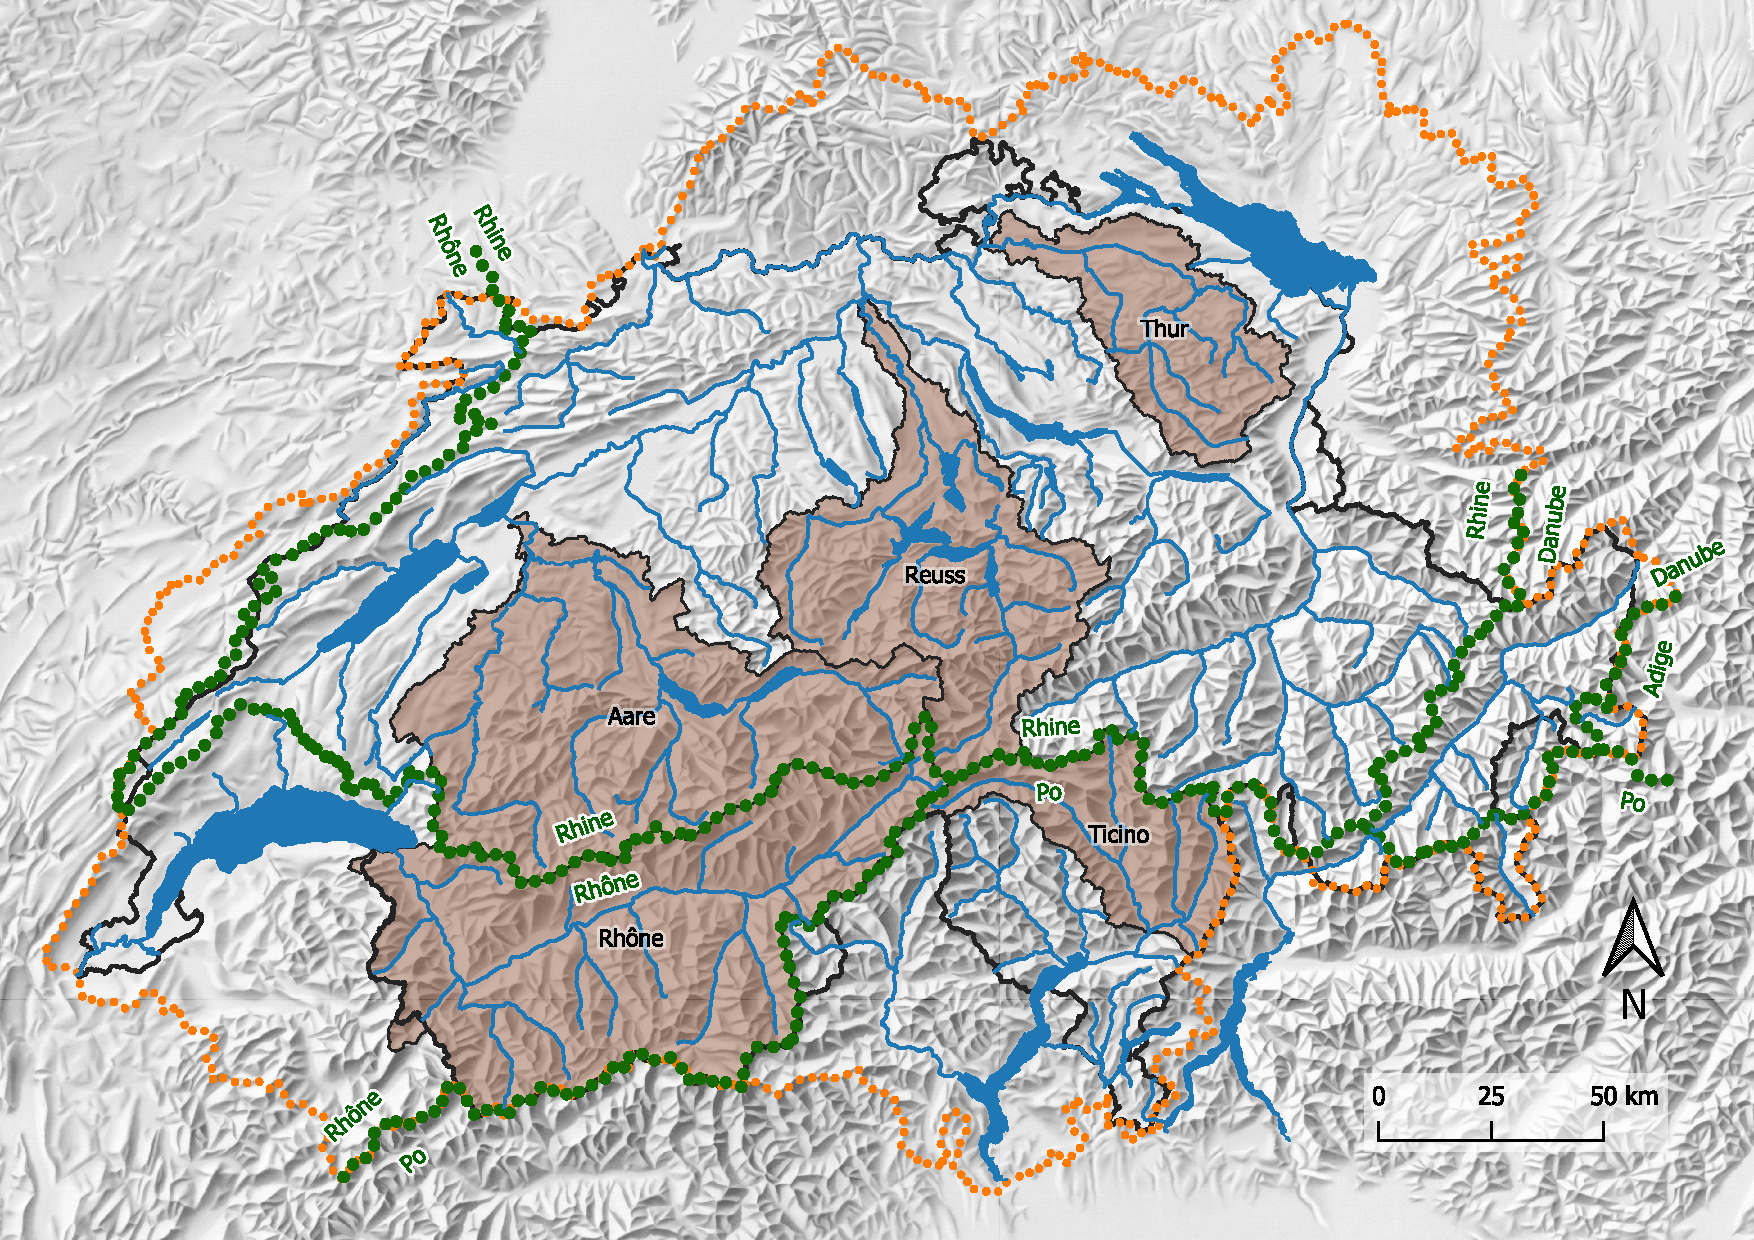
\includegraphics[width=0.95\columnwidth]{figures/map}
		\caption{{Map of Switzerland with its major drainage divides (green), the extent of the ``hydrological Switzerland'' (orange) and some catchments (brown) that are referenced in the text (Data: Federal Office of Topography swisstopo and Hydrological Atlas of Switzerland). \label{fig:map}
		}}
	\end{center}
\end{figure}


\subsection{Processes}
\label{sec:context:processes}


\subsubsection{Cryosphere}
\label{sec:context:cryosphere}

Contributions from snow and glaciers are key components of the alpine environment as they play a significant role in hydrological regimes through a temporal redistribution of water \citep{Barnett2005}. These processes thus need to be accurately represented in the models, which can be achieved with different levels of complexity. Most hydrological models used in Switzerland rely on a simple temperature-index based snow routine \citep[see for example][]{Jenicek2018}. On the other end, Alpine3D, which is built on the snowpack and ground surface model SNOWPACK (\citealt{Bartelt2002, Lehning2002a, Lehning2002b}), has undoubtedly the most complex representation of snow processes among Swiss models. It allows analyses that require a fully distributed simulation of mass and energy balance, such as the analysis of the influence of snow distribution and water transport within the snowpack on the catchment-scale hydrologic response \citep{Brauchli2017}, or the influence of snow processes on soil moisture and streamflow \citep{Wever2017}.

Despite of the relatively long history of development and application of snow hydrological models, detailed comparisons between simple snow routines and Alpine3D have not been conclusive so far in Switzerland, particularly in the context of climate change applications \citep{Kobierska2011, Shakoor2018}. It is noteworthy, however, that applications to extended periods remain challenging due to the high computational demand of Alpine3D, with only few attempts to complete long model runs \citep{Michel2021}. The only other hydrological model used in Switzerland that solves the energy balance to simulate snow accumulation and melt is one of the most recent versions of WaSiM; it solves the full energy balance and includes lateral redistribution of snow, but has seen a single application in Switzerland so far \citep{Thornton2021}. 

This quasi-dominance of a single snow model that resolves the energy balance at the Swiss level is comparable to the situation in other Alpine countries, e.g. in Italy \citep[Geotop;][]{Endrizzi2014}, in France \citep[Crocus;][]{Vionnet2012}, or Austria \citep[Admunsen;][]{Strasser2004}. This can certainly be explained by the substantial meteorological data requirements and the considerable effort required to develop and implement such models. This is nevertheless surprising given the importance of snow hydrological processes and related water resources for alpine countries \citep{Beniston2018}.

One possible explanation is the strong focus on the impact of glacier retreat on alpine hydrology, which is at the heart of many climate impact studies in Switzerland \citep{Horton2006, Schaefli2007b, Junghans2011, Addor2014, Finger2015, Etter2017}, and in alpine regions in general \citep{Huss2017}. In fact, most models developed in Switzerland have a glacier module to quantify the contribution of glaciers to the hydrological response of a catchment \citep[see for example][]{Finger2011, Verbunt2003, Zappa2007a, Uhlmann2013a}. 
 
However, in the past, all hydrological models used in Switzerland relied on simplified glacier retreat routines, even in the context of climate change impact simulations \citep[e.g.][]{Horton2006}. This gave rise to the development of the glacio-hydrological GERM model \citep{Huss2016, Junghans2011, Farinotti2012, Finger2013}; this model combines a simple snow-hydrological routine to a new glacier retreat parameterisation scheme, which is now widely applied internationally by the glacio-hydrological modelling community \citep[][called $\Delta$h-parametrisation]{Huss2010}. The awareness of the limitations stemming from poor representations of glacier dynamics in hydrological models is currently rising and further drives hydrological model development. An example is the implementation of the aforementioned $\Delta$h-parameterisation in HBV-light \citep{Seibert2018}. 


\subsubsection{Sediment production and transport}
\label{sec:context:sediments}
A particular topic that deserves a more detailed discussion is sediment production and transport. Despite of the importance of sediments in the alpine water cycle \citep{Hegg2006}, work in this field in Switzerland essentially focused on process observations \citep{Rickenmann2012}. Attempts were made to model sediment transport with the streamflow model PREVAH \citep{RaymondPralong2015}, but such studies fall short of accounting for sediment source dynamics and connectivity. The modelling of sediment sources, as well as transport capacity, requires complex models that yield reliable spatial patterns of hydrological processes. 

A single model has been developed for this purpose in Switzerland, TOPKAPI-ETH, which has been modified to account for river bed erosion and deposition processes using a sub-grid modelling scheme \citep{Konz2011}. This modification allows the simulation of erosion and deposition patterns, sediment transport rates, and evolution of the channel slope. \citet{Battista2020a} later developed a new soil erosion and sediment transport module for TOPKAPI-ETH to investigate the effects of precipitation and surface erodibility and their spatial variability on sediment fluxes, and to analyse the role of localised sediment sources \citep{Battista2020}. 

Sediment management, for example, in the context of hydropower production \citep{RaymondPralong2015, Gabbud2016}, is gaining importance in Alpine countries and might drive the development of new modules to simulate the interplay of hydrological and geomorphological processes at the catchment scale. 


\subsubsection{Ecohydrology}
\label{sec:context:ecohydrology}

Ecohydrology studies the feedbacks between ecosystems and the water cycle, at stream reach or catchment-scale \citep{Tague2020}. To date, catchment-scale studies with ecohydrological models accounting for feedback with vegetation are scarce in Switzerland. An early example is a work of \citet{Zierl2005}, who used the model RHESSys to study climate and land-use change impacts on alpine streamflow in Switzerland. Later, \citet{Fatichi2012, Fatichi2012a} developed an ecohydrological model, called Tethys-Chloris (T\&C), to simulate vegetation-hydrology interactions at large scales. It has been applied to catchments in Switzerland to study soil moisture spatiotemporal dynamics \citep{Fatichi2015a}, as well as to assess the vulnerability of Alpine ecosystems to climate change \citep{Mastrotheodoros2019}.

Another approach consists in coupling ecosystem models to distributed hydrological models, such as TOPKAPI-ETH for the analysis of the interactions between rivers, aquifers and ecosystems \citep{Foglia2009, Pappas2015}. In the context of simpler streamflow models, model coupling for ecohydrological purposes is limited to one-way coupling, as e.g. in the example of PREVAH that was coupled to a model for bedload transport and channel morphodynamics to assess climate change impacts on brown trouts \citep{Junker2015}. 

Most hydrological studies that analyse the interplay of vegetation and hydrology focus on the effect of land-use change by analysing different vegetation scenarios without modeling the actual feedback, in Switzerland as well as internationally \citep{Dwarakish2015}. We further discuss such land-use change studies in Sect. \ref{sec:context:climatechange}. Overall, catchment-scale ecohydrological studies remain rare in Switzerland, a situation that might change due to increasing awareness of human pressure on natural ecosystems and potential water use conflicts \citep{Milano2016}.


\subsubsection{Anthropogenic streamflow modifications and water quality}
\label{sec:context:infrastructures}

Anthropogenic impacts on water flow in the stream network are growing with expanding urbanisation and related hydraulic infrastructure, with efforts to produce more hydropower \citep{Schaefli2018} or with growing irrigation infrastructure. Related streamflow perturbations should not be ignored in hydrological modelling, but can be challenging to incorporate in a model due namely to the absence of detailed data on anthropogenic water use \citep{FOEN2021}.

In Switzerland, large hydraulic infrastructure is dominantly related to hydropower operations, including large dams and accumulation reservoirs and water diversions \citep{Schaefli2018}. Thus, specific modules have been implemented in several hydrological models, which in some cases simply led to model extensions, e.g. for WaSiM \citep{Verbunt2005} or TOPKAPI-ETH \citep{Fatichi2014}. Such model extensions were namely essential to analyse anthropogenic versus climate change effects on natural streamflow regimes \citep{Fatichi2014} or to anticipate hydropower operations in a climate change context \citep{Fatichi2015b, Anghileri2018}. One model developed in Switzerland has been specifically designed to simulate hydropower operations: RS MINERVE \citep{GarciaHernandez2020, Foehn2020}. The development of a specific model was considered necessary to simulate complex hydropower operations in the Valais region (upper Rhone catchment), which shows a particular high density of hydropower infrastructure.

Compared to hydropower, the main other water user, agriculture, has not received much attention in terms of hydrologic model development and streamflow simulation at catchment scale. A key reason might be that in Switzerland, limited water availability and potential droughts has only recently become an issue \citep{FOEN2021}. One example that we could find is the study by \citet{Fuhrer2012} that has shown that WaSiM is suitable to study the demand and supply of water for agriculture, including irrigation. In this area, models that are widely used internationally could be applied more in Switzerland. One such example is SWAT, which -- given its user-friendliness \citep{Abbaspour2007} -- could see more applications despite not being specifically designed for alpine environments \citep{Rahman2014, Andrianaki2019}. The need to model the feedback of agricultural water use and the catchment-scale hydrological response could lead to further hydrological model diversification; corresponding knowledge is currently missing in Switzerland \citep{FOEN2021}.

Future developments or applications of hydrological models specifically designed to reflect agricultural water use in an alpine context might in particular also be driven by the need to simulate corresponding water quality dynamics. Water quality studies at catchment-scale are, in fact, still rare to date in Switzerland. One example is the work of \citet{Abbaspour2007} who tested SWAT for modelling water quality and nutrient loads in the Thur catchment: they concluded that "in watersheds similar to Thur – with good data quality and availability and relatively small model uncertainty – it is feasible to use SWAT". Even the basic water quality variable, water temperature, has only received little attention in catchment-scale hydrology in Switzerland. It led to the development of an Alpine3D extension, Streamflow \citep{Gallice2016, Michel2021}.


\subsection{Applications}
\label{sec:context:application}


\subsubsection{Model improvement and uncertainty analysis}
\label{sec:context:uncertainty}

A large body of the international hydrologic modelling literature focuses on model performance with respect to reproducing observed streamflow \citep{Clark2011a, Beven2011}, e.g. as a function of model parameterisations \citep{GironsLopez2020}, of spatio-temporal model resolution \citep{Brunner2019}, of precipitation input data \citep{Sikorska2016, Sikorska2017, MullerThomy2019}, or parameter estimation techniques \citep{Foglia2009, Cullmann2011}. However, in the context of model diversity, this field of research has overall little impact because most modelling groups who work on such theoretical aspects often use their in-house models for proofs of concepts or to improve them (e.g. \citealt{Schaefli2007, Hingray2010}).

Model performance studies cover, for example, the integration of glacier mass balance data \citep{Finger2015, Schaefli2011}, snow data assimilation \citep{Griessinger2016}, accounting for streamflow observation uncertainty \citep{Westerberg2020}, the influence of spatial or temporal resolution of hydro-meteorological input \citep{GironsLopez2016, Felder2017, Sikorska2018}, integration of citizen science data \citep{Etter2020}, error correction in forecasting chains \citep{Bogner2018}, assessment of spatial pattern reproduction of soil moisture and evapotranspiration \citep{Rossler2010, Zappa2003} and of snow \citep{Zappa2008a}, and the comparison of various climate postprocessing methods \citep{Rossler2019}.

Overall, there are only a few parameter regionalisation studies, i.e. studies on the spatial transfer of model parameters, a key topic for hydrologic prediction in catchments without streamflow observations \citep{Guo2021}. On an international level, this question led to the development of specific models in conjunction with spatial parameter transfer approaches \citep[e.g., mHM;][]{Samaniego2010a}. In Switzerland, there was rather a focus on understanding the benefit of parameter regionalisation combined with few streamflow observations for the calibration of existing models and to counterbalance sparse operational observation networks especially in mountain areas \citep{Viviroli2015}.


\subsubsection{Characterisation and quantification of floods and droughts}
\label{sec:context:floodsdroughts}

Infrastructure planning, water resources and natural risk management heavily rely on probabilistic quantification of extremes, i.e. an estimation of what could happen in terms of floods and droughts and their associated probabilities (called return periods in hydrology). Work in this field continues to be based on statistical analyses and extrapolation of observed streamflow time series \citep{Brunner2018, Asadi20108}, but hydrological models play an ever-increasing role to complement missing or insufficient streamflow data.

Any model-based flood estimation method is computationally intensive since long model simulation runs are required at an hourly time step \citep[see][about reducing computational requirements for extreme flood estimation by hydrological modelling]{SikorskaSenoner2020}. Accordingly, simple models such as PREVAH \citep{Viviroli2009, Viviroli2009c, Felder2017}, HBV-light \citep{Sikorska2017, Brunner2019a, SikorskaSenoner2020} and  RS MINERVE \citep{Bieri2013, Zeimetz2017, Zeimetz2018} are often used for flood estimation; these models are all deemed to perform well enough for flood estimation in Swiss catchments by their respective authors and users. Furthermore, at the time of writing, the open-source DECIPHeR model is further developed and implemented for Swiss catchments to bring diversity in the type of models used for flood modelling (Kauzlaric, personal communication).

Other more complex distributed models are also used for flood modelling, but more often on an event-based scale, as in the case of a reconstruction of the 1816 Tambora eruption and its impact on floods in the upper Rhine basin with WaSiM \citep[see Fig. \ref{fig:map};][]{Rossler2018}. Such a model can be highly relevant to study specific flood types that involve a detailed description of small scale processes, such as to analyse  rain-on-snow flood events \citep[][with WaSiM]{Rossler2014} or the interplay of rainfall temporal variability and the clustering of saturated areas \citep[][with TOPKAPI-ETH]{Paschalis2014}

Work on droughts is much less abundant in Switzerland than work on floods, which is related to the fact that missing water was, in the past, not a hot topic in this country known as the water tower of Europe \citep{Milano2015}. What can be highlighted here is that the same models are in use to assess droughts and floods, potentially with specific recalibration, but without modification of the model structure. This is motivated by the fact that existing models are deemed to reproduce well all dominant processes in the Swiss environment, as, e.g., explicitly stated in the work of \citet{Zappa2007a} on quantifying the hydrological impact of the 2003 heatwave with a distributed version of PREVAH. It was also later on used for additional drought analyses \citep{Brunner2019e, Zappa2019}, where a spatial mismatch between water scarcity and storage availability has been highlighted for Switzerland \citep{Brunner2019e}. 
Similarly, HBV-light served in several drought studies, such as for the definition of a new drought index that accounts for snow \citep{Staudinger2014}, the predictability of low flows \citep{Staudinger2014a}, or the sensitivity of catchments to meteorological droughts \citep{Staudinger2015}. It was also used to assess low flow drivers in Alpine catchments \citep{Arnoux2020}. However, significant efforts to improve the representation of groundwater and the corresponding baseflow during droughts remain to be done in Switzerland, which might lead to further model development or diversification.


\subsubsection{Climate change and land-use change impact analysis}
\label{sec:context:climatechange}

Climate change impact studies emerged in Switzerland in the 1990s, including a large national research programme on climate change and natural hazards \citep{SNFS2021}. Since then, all model-based studies are mostly conducted with the models that established themselves in Switzerland, which have, however, not been specifically designed for climate change impact analysis; detailed assessments of how well these models can simulate future conditions are largely missing. Climate change impact analyses require, among others, a good representation of the processes that play a key role in the studies. The representation of these processes in the models is discussed in Sect. \ref{sec:context:processes}, both for present and future climate conditions. These studies also require models that are not too time-consuming due to processing of long transient periods as well as due to the increasing ensemble size of modelling chains.

WaSiM was chosen by \citet{Middelkoop2001} for a climate change impact study primarily due to its good interpolation of meteorological data for mountain environments, and by \citet{Jasper2004} to assess the effect of different regional climate scenarios in the Thur and the Ticino catchments (Fig. 1). WaSiM has also been applied to assess future soil water patterns \citep{Jasper2006, Rossler2012} and future summer evapotranspiration regimes \citep{Calanca2006}, applications where a spatially detailed representation of vertical and horizontal flow processes -- involving the Richards equation -- is important. It was even applied for the entire Rhine basin at a 1~km\textsuperscript{2} resolution down to Rotterdam by \citet{Kleinn2005}.

TOPKAPI-ETH, the other frequently used fully distributed model with explicit simulation of horizontal and vertical fluxes, has also been applied to several climate change impact studies, such as in the analysis of internal climate variability \citep{Fatichi2014}, or the assessment of future water resources \citep{Finger2012}. It was also selected by \citet{Fatichi2015}, who argues that "it represents a reasonable compromise between physically meaningful representation of hydrological processes and computational time for large-scale ($>$1000~km\textsuperscript{2}), long-term ($>$20~yr), high-resolution ($<$1~km\textsuperscript{2}) distributed simulations".

However, the most widely used models to study climate change impact on streamflow are to date the so-called reservoir-based models PREVAH (\citealt{Koplin2012, Speich2015, Milano2015a, Brunner2019c} and others;  see Supplementary material) and HBV-light (\citealt{Etter2017, Hakala2020, Brunner2018a, Jenicek2018}  and others). In the western part of Switzerland, RS MINERVE and GSM-SOCONT have been used, especially for high elevation sites \citep{Horton2006, Uhlmann2013a, Uhlmann2013b, Terrier2015}. The rationale for using these models is well summarized by \citet{Koplin2010} who, for PREVAH, states that the model ``has been developed especially to suit conditions in mountainous environments'' and that it ``has proved to be a reliable and flexible tool for various scopes of application and climate conditions ranging from drought analysis over water balance modelling to flood estimation and forecasting''. 

One point to note is that the adequacy of the models to a different climate is generally not discussed. References to previous studies are sometimes provided, without the latter having addressed this point explicitly. While it is relatively easy to demonstrate a model's ability to reproduce floods or drought conditions, its transferability to other climate conditions is more difficult to prove directly and generally not tackled (see Sect. \ref{sec:multi-model}). 

Compared to climate change impact analysis, land-use change studies are rare in Switzerland and did not lead to the development of specific models or model extensions so far. Examples are the work on the effect of forest change by \citet{Koplin2013} and \citet{Schattan2013}, both with PREVAH or by \citet{Alaoui2014} with WaSiM. This absence of detailed land-use change studies might be explained by the dominance of climate change impact studies over the last few decades. 


\subsubsection{Operational forecasting}
\label{sec:context:forecasting}

The ever increasing need for reliable real-time streamflow forecasts leads to a continuous evolution of the underlying hydro-meteorological modelling systems. Operational forecasting started with deterministic forecasts from a single meteorological forecast applied to a single hydrological model; today, users expect full probabilistic ensemble forecasts at hourly time scales, updated every few hours and with several meteorological inputs applied to different hydrological models \citep{Jasper2016}. Coupled atmospheric--hydrologic ensemble prediction systems were proven to provide better forecasts than deterministic simulations \citep{Verbunt2007, Zappa2008, Jaun2008, Liechti2013}. These might also include data assimilation schemes \citep{JorgHess2015a} or the assessment of hydrologic uncertainty related to meteorological forcing, model parameters and initial conditions \citep{Jaun2009, Zappa2011a, Fundel2011}.

Such modern forecasting systems require hydrological models that provide forecasts at many locations in a stream network, and that includes the effect of hydraulic infrastructures (e.g., of hydropower water intakes and accumulation lakes, see Sect. \ref{sec:context:infrastructures}). Since the early times of flood forecasting in Switzerland, HBV and PREVAH were used in governmental offices \citep{Jasper2016} as well as in research institutes because of their relative simplicity and low computational costs \citep{Verbunt2006, Addor2011, Murphy2019, Antonetti2019}. Along with HBV, PREVAH and LARSIM, WaSiM is today part of the Swiss operational ensemble forecasting system \citep{Jasper2016}, which uses the FEWS platform (Flood Early Warning System; \citealp{Werner2013}) to provide forecasts for the cantonal authorities and the public \citep{FOEN2019}. A key advantage of the WaSiM model is that it can explicitly account for lake regulations and hydropower operations (J. Schulla, personal communication, October 23, 2020). WaSiM has also been used for research studies on improving operational flood forecasting in mountainous areas \citep{Jasper2002, Jasper2003, Ahrens2003a, Ahrens2003b}.

In parallel to the models mentioned above, RS MINERVE is being used as a specific flood forecasting tool for the upper Rhone river catchment, a large catchment (5220 km\textsuperscript{2}, see Fig. \ref{fig:map}) strongly influenced by glacier melt and hydropower production \citep{GarciaHernandez2009b, GarciaHernandez2009, Jordan2010}. The model has been primarily developed for this application. Furthermore, its interpolation of the meteorological forcing and its partitioning between rain and snowfall have been enhanced to improve the forecasts in this catchment \citep{Tobin2011, Tobin2012}.

Applications or studies of subseasonal to seasonal (lead times up to 4 to 6 weeks) streamflow forecasts are relatively scarce in Switzerland, but few applications using PREVAH exist \citep[][]{Monhart2019, Anghileri2019}. PREVAH also plays a prominent role in operational drought forecasting \citep{Fundel2013, JorgHess2015, Bogner2018b} and within the operational Swiss drought information platform (\citealp{Stahli2013}). 


\subsubsection{Large scale modelling}
\label{sec:context:largescale}

To complete the picture, we address here the application of some international hydrological models implemented for Europe or large European river basins such as the Rhine and thus covering at least a significant part of the hydrological domain of Switzerland (Fig. \ref{fig:map}). However, we restrict ourselves to those models whose code is publicly available and/or whose results are published and/or directly available for Swiss basins.

\citet{Kauffeldt2016} presented a technical review of large-scale hydrological models with regard to their suitability for the European Flood Awareness System (EFAS). Specific criteria must be met for a model to be suitable for continental-scale forecasting, such as a representation of all major processes in the domain, flexibility in resolution and spatial discretisation, a possibility for data assimilation, etc. \citep{Kauffeldt2016}. Amongst the models evaluated in the study, three have been specifically deployed for Europe: LISFLOOD, HYPE and mHM (see Appendix 1). While LISFLOOD and HYPE (or E-HYPE for the version covering the pan-European continent) are already running operationally (see Appendix 1) at the European scale, mHM has only recently been applied for the development and evaluation of a pan-European multi-model seasonal hydrological forecasting system \citep{Wanders2019}.

Several other models have been applied specifically for the Rhine basin, mainly focusing on forecasting discharge or climate change impact applications. Examples include the so-called wflow\_hbv model (\citealp{vanOsnabrugge2017}, \citealp{vanOsnabrugge2019} and \citealt{vanOsnabrugge2020}) for hourly/daily streamflow forecasting of the Rhine, allowing lake level data assimilation. Another example is the LARSIM model, which was implemented at a 1~km\textsuperscript{2} resolution in combination with HBV-light to assess the origin of streamflow components \citep{Stahl2017}. The major regulated and unregulated lakes were included in LARSIM, as well as four of the most influent ``clustered'' hydropower reservoirs present on the upper Aare, upper Reuss, upper Rhine, and in the Ill river catchment (Fig. \ref{fig:map}).

In general, the skill of most large scale models is found to be inferior near the main Alpine ridge compared to mountainous or lowland areas. The high Alpine catchments have been identified early as posing a major challenge to large scale hydrological modelling \citep{Kleinn2005}.  Besides larger errors in the meteorological variables (precipitation in particular) and the important effect of water management practices, the smaller the catchment area and the greater the elevation ranges, the more detailed the model structure and the spatial resolution need to be to achieve good model performances \citep{Gurtz2003}. While most likely being cancelled out downstream \citep{Kleinn2005}, these problems remain yet to be addressed in large scale modelling and certainly partly explain why specific Swiss-scale models continue to be extremely popular. 


\section{The motivations behind the model choice}
\label{sec:motivations}

In total, we reviewed 157 peer-reviewed journal articles on hydrological modelling in Swiss catchments (see Table 1 in the Supporting Information). Excluding the large scale applications (Section \ref{sec:context:largescale}), a Swiss hydrological model (category D or E in Table 1) is selected in 93\% of cases, leaving little room for international models. PREVAH takes the lion's share with about 30\% of the applications, followed by HBV-light (16.5\%) and WaSiM (14.6\%). The most used international model is SWAT with a small 4\% usage (7 cases), mainly related to research led from outside Switzerland.

As depicted in Sect. \ref{sec:context}, some models are specialised for certain processes, such as Alpine3D for snow and GERM for glaciers, and are thus proportionally more used in these contexts (Fig. \ref{fig:applications}). TOPKAPI-ETH tends to be more used for applications that require a spatially-distributed output of horizontal and vertical fluxes, e.g. in view of coupling to another model. RS specifically targets flood modelling and hydropower operations, as it was designed for operational flood mitigation with hydropower plants. The three most used models, i.e. PREVAH, HBV-light and WaSiM, are general models and are applied to different topics, such as climate change impact studies, floods, droughts, cryosphere-related processes, and operational forecasting (Fig. \ref{fig:applications}).

\begin{figure}[htb]
	\begin{center}
		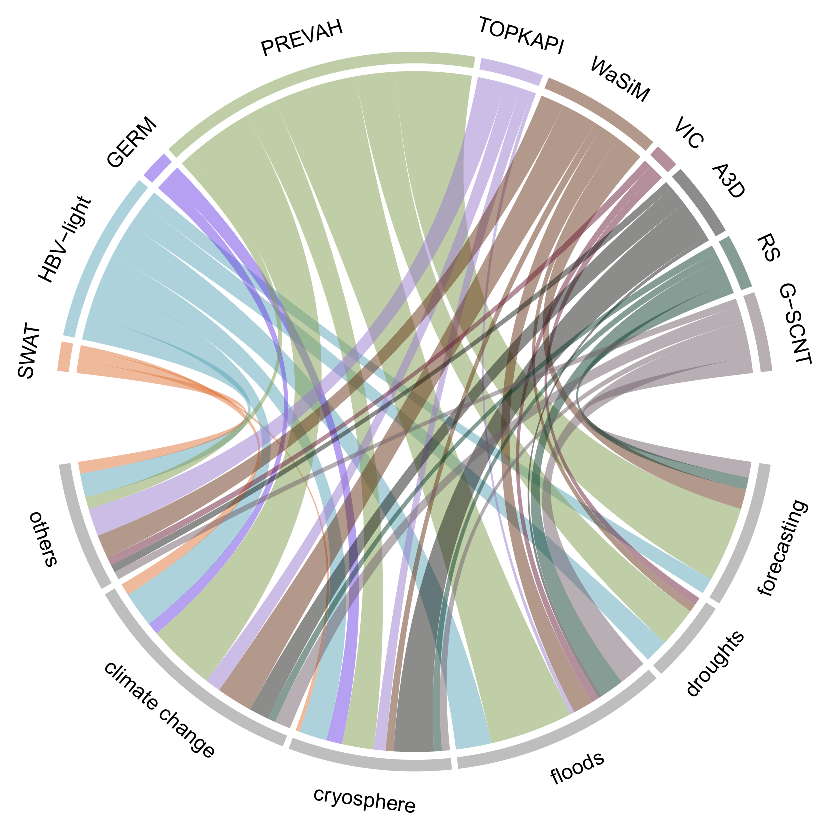
\includegraphics[width=0.70\columnwidth]{figures/chord_diagram_contexts}
		\caption{{Hydrological models applied to different contexts in Switzerland. The importance of the link is proportional to the number of scientific articles. The importance of some models can be inflated by the fact that an article can address multiple contexts, such as floods and climate change. Models with too few use cases (less than three) are not included for the sake of clarity. A3D stands for Alpine3D and G-SCNT for GSM-SOCONT. 
		{\label{fig:applications}}
		}}
	\end{center}
\end{figure}

In the analysed articles, about 25\% of the authors specifically address the model's adequacy with the context or the landscape. However, this does not mean that adequacy has been formally tested or that it actually drove the choice of the model, but rather that the model is argued as suitable to the intended application. About 53\% of the articles do not mention the adequacy of the model to the context. The rest provide some description of the model characteristics that might be interpreted as arguments for suitability to the case study. Furthermore, there are only few examples where the authors explicitly discuss their perceptual model \citep{Beven2021}, i.e. their perception of how nature works, which is generally left to papers dedicated to model development.

Other factors than adequacy can drive the model choice: some of a practical nature and others of a more subjective nature. \citet{Addor2019} argue that the choice of a model is driven by legacy rather than adequacy, where by legacy they understand: ``practicality, convenience, experience, and habit''. This can include, on the one hand, the experience available in the modelling group and, on the other hand, code and data availability. Some of these practical aspects are not reflected in the literature: Peer-reviewed articles involve a reshaping of the narration \citep{Pontille2007, Rinck2010, Babel2019}, i.e. the chronology of decisions is often modified to fit a standard paper structure and the drivers behind the decisions are adapted retrospectively. The practical aspects that drove model selection are thus difficult to assess objectively without additional information. For that reason, we conducted a survey inviting all first authors of the analysed papers to participate, as well as other actors in the research community actively using hydrological modelling approaches in Switzerland. About 100 persons were contacted, and 50 took part in the survey. The web-based survey could be completed anonymously.

The survey started with four general questions on the experience of the researcher in the domain of hydrological modelling and model development (Fig. \ref{fig:survey_general}). The objective of this first part was to provide a context to the answers given in the rest of the survey. The survey then included multiple-choice questions (Fig. \ref{fig:survey_histograms}) addressing the choice of the hydrological model used by the researcher for previous work (14 questions), the factors that the researcher would nowadays consider important in model selection (nine questions), and finally, the researcher opinion on multi-modelling approaches (four questions; treated at Sect. \ref{sec:multi-model}). The answers shown in Fig. \ref{fig:survey_histograms} have been stratified based on the model development experience of the researcher (Fig. \ref{fig:survey_general}d). The stratification based on experience was most relevant compared to the others.


\begin{figure}[htbp]
	\begin{center}
		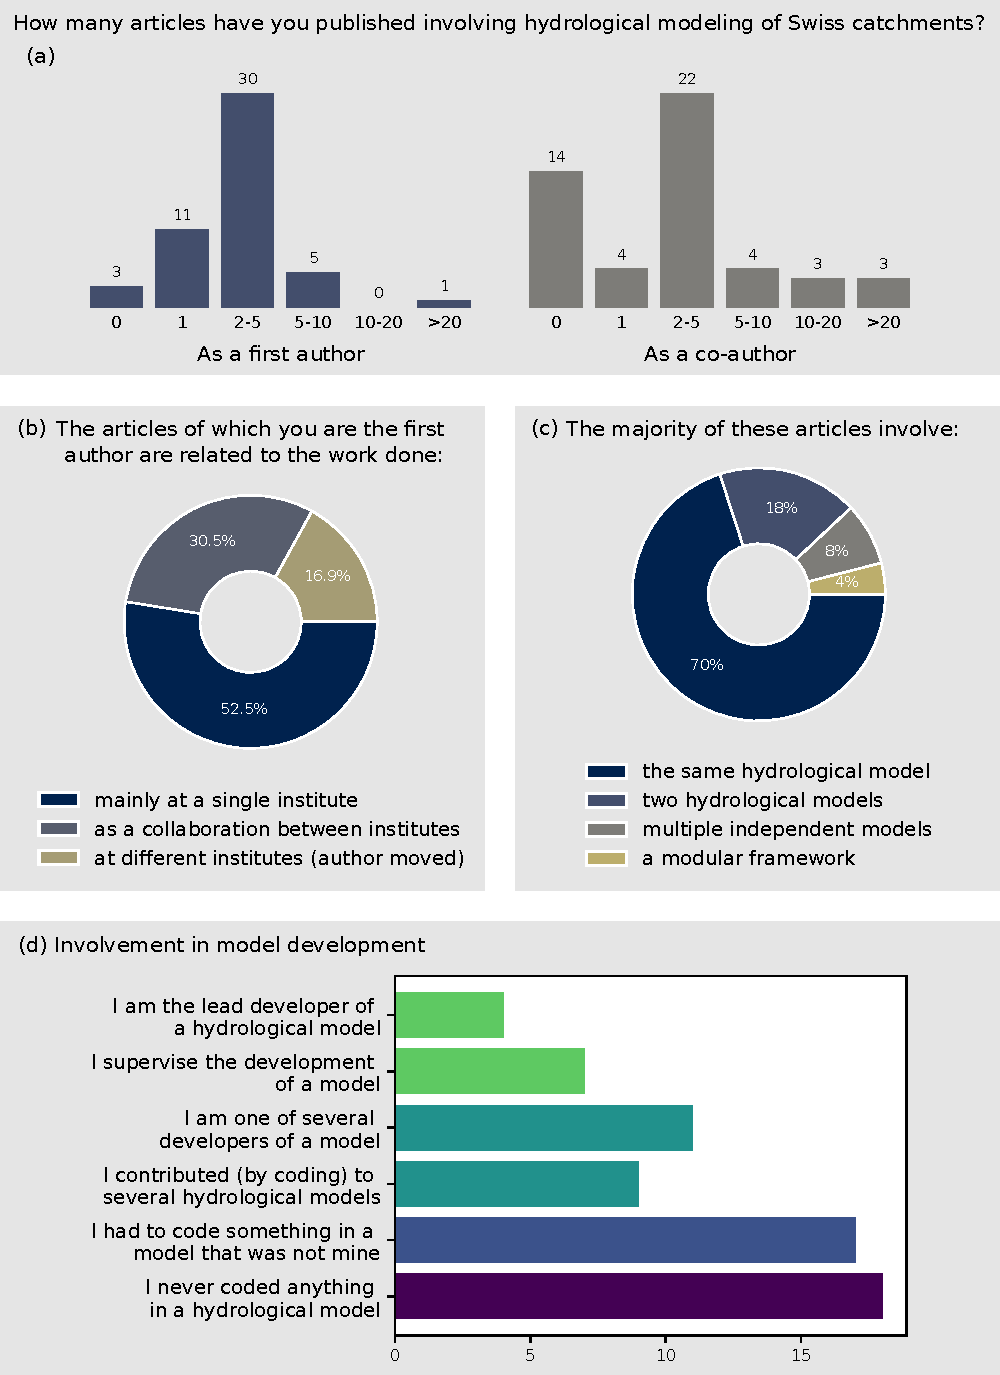
\includegraphics[width=0.90\columnwidth]{figures/survey_general.pdf}
		\caption{{Survey results: answers to the general questions.
		{\label{fig:survey_general}}
		}}
	\end{center}
\end{figure}


\begin{figure}[htbp]
	\begin{center}
		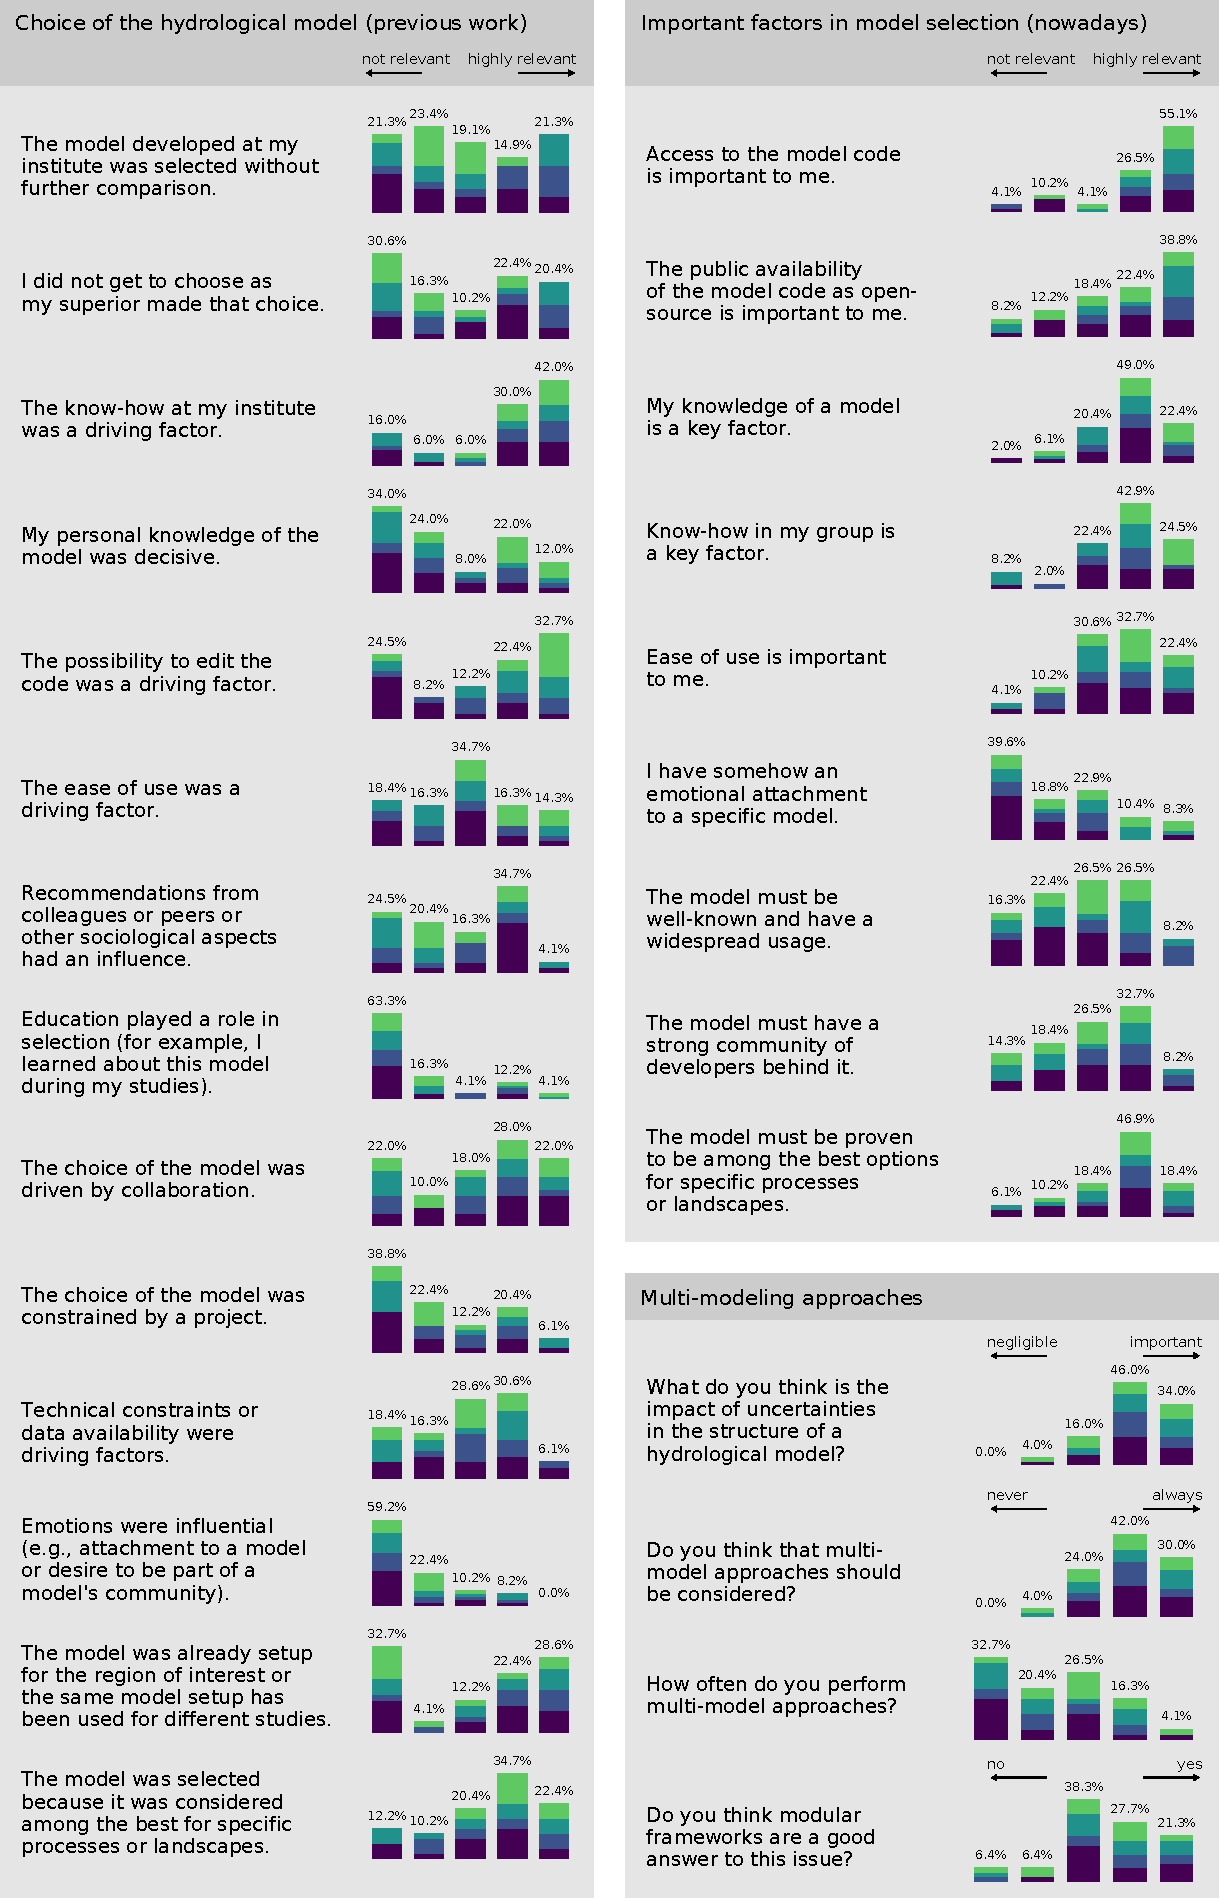
\includegraphics[width=0.90\columnwidth]{figures/survey_histograms.pdf}
		\caption{{Results for the survey questions about model selection. The histograms have been stratified based on the involvement of the researcher in model development (Fig. \ref{fig:survey_general}d). As the question on the involvement offered multiple selections, the stratification was performed according to the hierarchy of Fig. \ref{fig:survey_general}d, and researchers were thus assigned to the highest selected class. 
		{\label{fig:survey_histograms}}
		}}
	\end{center}
\end{figure}


We first look at the effect of the host institutions of the first author. About half (52.5\%) of the researchers stayed at the same institute when they published -- as first author -- most of their articles on hydrological modelling (Fig. \ref{fig:survey_general}b). In such a case, the model choice is likely strongly biased in favour of the model developed and used at the corresponding research institute \citep{Addor2019}. Indeed, in 66\% of analysed articles, the first author is affiliated with the institute where the chosen model is being developed. When asked if the model developed at the institute was chosen without further comparison, the researcher's opinions differed (Fig. \ref{fig:survey_histograms}). While 36.2\% agreed with that statement (the percentage of agreement is defined here as the sum of the frequency of the two positive categories, i.e. "relevant" and "highly relevant"),  44.7\% did not agree, including both non-developers and researchers mostly involved in model development. Researchers with less development experience were also more influenced by their superior when it came to the model choice than researchers with more experience. 72\% of all researchers considered know-how at the institute as a relevant driver for previous work (67.4\% for the present situation), significantly more than the personal knowledge of a model (which, however, seems much more important for the present situation). The strong link between the institutes and some models (see also Fig. \ref{fig:model-institutes}) brings the advantage that the model at hand is thus well known, that the code is available, and that specialists for potential modifications are present. All of these factors are a positive aspect, as in-house experience (or habits) can contribute to efficiency and expertise \citep{Babel2019}. Care has to be taken that habits do not come at the expense of adequacy. The risk of habits lies in the automatism of our decisions \citep{Babel2019}, and in the Hammer and Nail syndrome ("if all you have is a hammer, everything looks like a nail"), i.e. a researcher will seek to solve every problem with the known model \citep{Hamalainen2015}.

\begin{figure}[htb]
	\begin{center}
		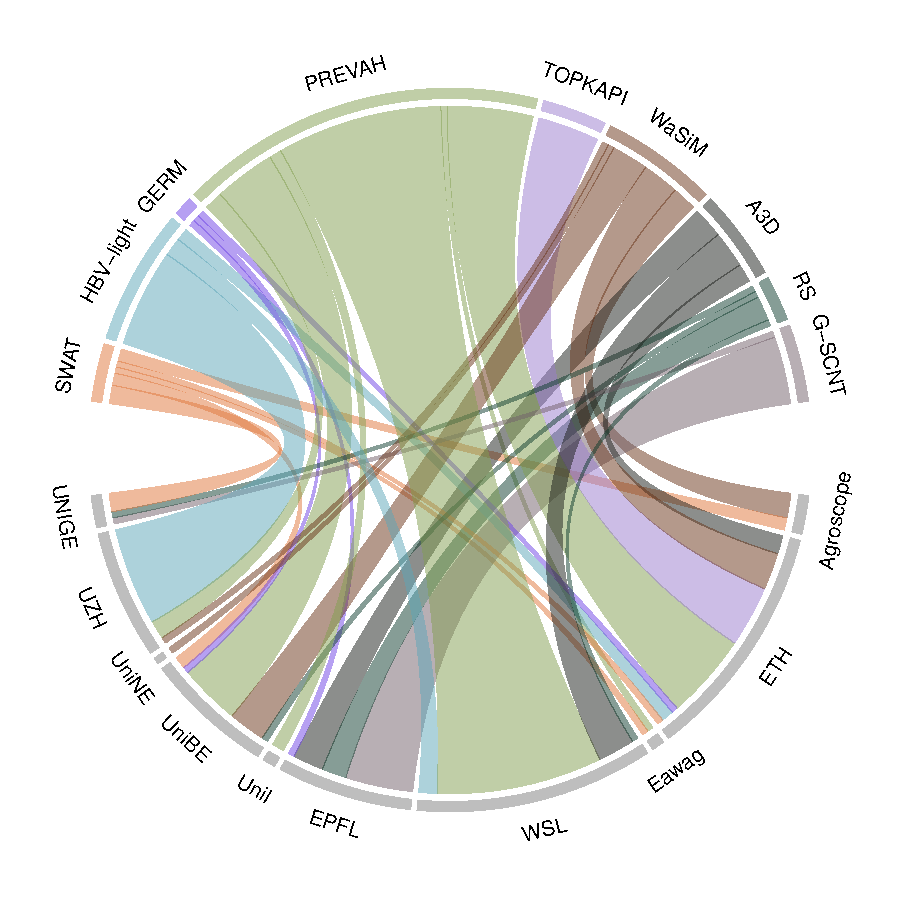
\includegraphics[width=0.70\columnwidth]{figures/chord_diagram_institutes}
		\caption{{Links between hydrological models and the Swiss institutes that use them. Same conventions as Fig. \ref{fig:applications}. Models or institutes with too few use cases are not included.
		{\label{fig:model-institutes}}
		}}
	\end{center}
\end{figure}

When the chosen model is not developed at the institute where the research is conducted, collaborations are often established with the model developer or lead researcher. Consequently, the model developer (or team leader) is co-authoring the paper in 72\% of the published articles. Survey results also show that collaboration was a driving factor for 50\% of the researchers (Fig. \ref{fig:survey_histograms}). Another reason driving the hydrological model choice is the reuse of a model already set up for a catchment of interest, sometimes without the need to recalibrate it. About 20\% of the articles explicitly state that the applied model comes from another study. This number should likely be higher, as some authors publish multiple articles targeting different topics using a single model setup without explicitly mentioning it. The survey revealed that 51\% of the researchers agreed that model setups had been reused (Fig. \ref{fig:survey_histograms}).

Access to the model source code has been qualified as a relevant driving factor by 55.1\% of the researchers for previous work, unsurprisingly with a clear contribution from model developers (Fig. \ref{fig:survey_histograms}). This number even increases to 81.6\% for the current situation, which reveals a strong desire to be able to edit the model code to adapt it when necessary. However, despite of access to the source code, researchers do not necessarily modify it. This might also partly be a psychological factor, i.e. people feel more secure to invest time and energy in a model that they know they can eventually adapt, rather than being stuck in a situation where they cannot modify the model code. Although access to the model code is important to many authors, it does not mean that everyone sees the necessity of public availability (as open-source) of the model code. Indeed, 61.2\% of the researchers considered the public availability of the model code as important to them, which is high, but less than 81.6\% of researchers who would just like to have access to the code. Some models have been open-source for a long time, such as VIC or FUSE \citep{Clark2008}, but either were used very sporadically for an individual catchment -- generally by foreign institutions -- or have not yet been used in Switzerland.

Adequacy to specific processes or landscapes was considered as important in model selection by 57.1\% of the researchers for past studies and by 65.3\% for the current situation (Fig. \ref{fig:survey_histograms}). Ease of use does not seem to have had a substantial impact on model selection in the past (30.6\%) but would be more important today (55.1\%). Technical constraints and data availability (36.7\%), or project-related constraints (26.5\%) had a moderate impact. Today's opinions differ regarding the importance of a widespread usage of a model or the existence of a strong community of developers behind it. 

External factors also influence the model choice. While education seems to play only a marginal role, sociological aspects, such as recommendations from colleagues or peers, have a non-negligible impact (38.8\%), mainly among researchers not involved in model development. \citet{Babel2019} showed, based on interviews with model developers, that the choices made during model conception and development can be indirectly influenced by various actors. Some transferred knowledge becomes self-evident for the developer, who embraces external influences. This process of incorporation of external influences is also likely to impact the model choice.

Finally, emotions are not stated as a key factor, mainly for past work. We would have expected a stronger signal of personal attachment of the developers to their model. The survey terminology was maybe not appropriate here, leading to biases in the answers. Other terms, such as 'familiarity' or 'confidence' might have led to different results. This dimension is highly subjective, and we dare to suggest that this subconscious driver is more important than stated on the survey answers, mainly for developers invested in a specific model. Indeed, \citet{Chamberlin1890} shows that people tend to develop a parental affection for their theories, which can be transposed to models, and which hinders recognition of the benefits of other approaches. Moreover, emotions were shown to play a significant role in decision making and can be seen as "invisible actors in the system of problem solving" \citep{Hamalainen2015}.


\section{On model structural uncertainty and multi-model approaches}
\label{sec:multi-model}

The World Meteorological Organization (WMO) used to carry out comparisons of hydrological models and publish the results in Operational hydrology reports \citep{WMO1986, WMO1992a}. In this context, different international models were compared over various catchments, including the Dischma basin in Switzerland. The Snowmelt Runoff Model \citep[SRM,][see supplementary material]{Martinec1975} has also been assessed in these early model comparisons \citep{WMO1986, WMO1992a}.

Since then, few model intercomparison studies have been conducted in Switzerland. The existing ones are studies on what we can gain from model complexity in terms of model performance. For example, \citet{Gurtz2003} compared PREVAH and WaSiM for two mountainous catchments, showing that, despite of their significant complexity difference, both models show a similar performance in terms of streamflow simulation. This result was also reproduced in the study by \citet{Orth2015} comparing HBV-light, PREVAH, and an even simpler model, but with performance varying depending on the considered hydrological variable or hydrological conditions. They highlighted that that there is no single model that is best suited to all hydrological conditions.

Similarly, few studies are relying on a multi-model approach to predict future hydrologic behaviour. The use of multiple hydrological models aims at accounting for the uncertainty associated with the models' structure, their numerical implementation, and their processes representation. The idea is to consider a diversity of models that represent the uncertainty at play \citep{Babel2019}. Such multi-model approaches are in particular extremely relevant for probabilistic flood forecasting \citep{Kauffeldt2016} or for long term climate change impact predictions \citep{Kobierska2011, Kobierska2013, Andrianaki2019}, where different model formulations can lead to different model sensitivities with respect to the climate forcing and thus to different results. 

In the context of climate change impact analysis, multi-models are in fact of key importance to understand the dominance of different uncertainty sources, i.e. those related to the climate change scenarios and those related to the hydrological modelling itself. \citet{Bosshard2013a}, for example, showed that none of the uncertainty sources they assessed is negligible, and that the respective contributions to the uncertainty vary over the year with a larger contribution from the hydrological model in winter and spring. Similarly, \citet{Addor2014} assessed the impact of climate change on hydrological regimes comparing models of different complexity (HBV-light, PREVAH, WaSiM) for six catchments in Switzerland. The hydrological models contributed significantly to the overall climate change impact uncertainty in the (partially) glacierized catchments. This finding was reproduced in the recent re-evaluation of climate change impacts on Swiss hydrology \citep[Hydro-CH2018,][]{FOEN2021} with a similar hydrologic model ensemble (HBV-light and two different versions of PREVAH). It showed that the largest relative differences between the models occur especially in glaciated or high-elevation catchments in the low flow seasons (winter and spring) or in summer in terms of absolute differences in simulated streamflow.

It is noteworthy that in all these studies, it was assumed that the parameters calibrated for the present conditions also apply in the future. As shown by \citet{Melsen2021} for 605 catchments in the United States with the models SAC \citep[Sacramento Soil Moisture Accounting model;][]{Burnash1973}, VIC, and HBV, this is an important and specific uncertainty factor in climate change impact modelling chains, but how to address this question remains one of the key challenge for hydrological modelling, and has not seen any specific developments in Switzerland so far. 

Overall, multi-model studies are still rare in Switzerland. This is in strong contradiction with our survey, which revealed that 80\% of the researchers considered the impact of the model structure as an important source of uncertainty, and 72\% supported that multi-models should be considered (Fig. \ref{fig:survey_histograms}). However, only about 20\% claimed to do it regularly, while 53\% admitted to (almost) never do it. The first reason given for not doing multi-model approaches is the lack of resources (time or/and money) for such exercise (supported by 76.6\% of the participants). The second reason is that it requires too much effort to set up another model (61.7\% of the participants); the third one is that other sources of uncertainty are considered more significant (40.4\%), and the fourth is related to the lack of know-how of another hydrological model (31.9\%). In addition, other reasons were provided, such as the carbon footprint of simulations and thus the need to do as few simulations as possible with improved models or the difficulty to interpret the results. Other participants suggested working with a single model but testing multiple structures and parameter values or working with model variants (such as \citet{GironsLopez2020}, who tested numerous snow routines with different degree of complexity).

Researchers are used to work with a single hydrological model (70\% of the survey participants; Fig. \ref{fig:survey_general}) and rarely learn to use another model. As discussed above, the use of another hydrological model requires a substantial effort. An eased assessment of multiple structures is the objective of the so-called "modular modelling frameworks" (used only 4\% of the time by the survey participants), strongly encouraged by \citet{Clark2011a}. Modular modelling frameworks allow hypothesis testing by generating models using different modules and variants of numerical implementations \citep{LaFollette2021}. Nowadays, several of these frameworks exist, such as SUPERFLEX, FUSE \citep{Clark2008}, PERSiST \citep{Futter2014}, ECHSE \citep{Kneis2015}, MARRMoT \citep{Knoben2019}, Raven \citep{Craig2020}, and SUMMA \citep{Clark2015}. Such modular frameworks can favour the generation and testing of new hypotheses about dominant hydrological processes and how to encode them in models. An example in Switzerland is given by \citet{DalMolin2020}, who discusses, based on the SUPERFLEX framework, how to flexibly adapt the model structure to integrate new hypotheses about dominant hydrological processes. 

Modular frameworks have theoretically the potential to counter-act model diversification, since they assemble different model structures in a single framework. The current experience and the survey show, however, that modular frameworks are not easily adopted by the modelling community. 


\section{Discussion and conclusion}
\label{sec:conclusion}

Focusing on Switzerland, we carried out a comprehensive literature review on hydrological models developed and applied in different contexts. The objective of this work was to disentangle the motivations and reasons behind the choices that led to the current co-existence of a wide range of streamflow models, even at the scale of a small country. To structure the analysis, we attempted a classification into process-driven and application-driven influences. For all reviewed studies, we examined the arguments for model selection that were explicitly put forward by the authors, as well as implicit aspects, such as the author's affiliation or co-authorships. Additionally, a survey was conducted among the authors and other actors in hydrological modelling in Switzerland to better assess more subjective drivers.

A key result of the literature review is the fact that published work crucially lacks adequately addressing model adequacy for the study context or the landscape, which partly hinders objective insights into decision processes involved in model choice. Additional insights from the web-based survey reveal that model adequacy to the analysed landscape is of foremost importance for model developers and users, which at least partly explains the lack of adoption of international or large-scale models. 

Researchers active in Switzerland are, in fact, very keen on using local models, either developed in Switzerland (93\% of the case studies) or even at their own research institute (66\% of the articles analysed). This strong link between models and institutes provides the benefit of expertise and efficiency, but at the risk of context inadequacy for the selected models and of automatism in decisions \citep{Babel2019}. Also, research groups have models configured for certain catchments and reuse them for different studies. This helps be more efficient and allows focusing on the main goal of a specific study, as long as the setup is appropriate for the application. Small projects might not have the resources to compare models and select the best one for a given context. This model-institute link is likely to be one of the main causes of the existence of so many hydrological models, since each research group develops its own tools. There may also be emotional aspects involved, such as the attachment of teams/users/developers to their model, that were not accurately identified by the survey due to terminology issues that could have biased the results.

These drivers of model diversity certainly depend on local specificities, such as the alpine context or Switzerland's strong focus on climate change impact analysis or energy production. The key findings of our study are however readily transferable to other contexts or scales: a foremost driver of hydrologic model diversity is the use of local models, to benefit from local know-how as well as to maximize model adequacy to the analyzed landscape. Modelling contexts and landscapes might change, but our scientific, practical, and financial incentives or constraints are pulling us in the same direction.

It is important to underline here that hydrological model diversity is interesting to represent the uncertainty related to the hydrologic model structure or implementation \citep{Babel2019} and that there will never be a single model valid for all applications \citep{Hamalainen2015}. However, in Switzerland, multi-model applications to harness this diversity are largely missing. A first barrier to this approach is the challenge to master multiple models. In this regard, modular modelling frameworks could help to move in this direction, but our review shows that they are not easily adopted.

This lack of multi-model studies is in contradiction with the importance that is attributed to such studies in our author survey. This finding is certainly transferable to the larger international modelling community. Many of us advocate the development of methods that facilitate robust model development \citep{Zheng2018}, but most of us do not apply these principles ourselves. This contradiction between what we think that we should do (multi-model analysis) and what we actually do (use our local model) might be partially related to research funding, in Switzerland and elsewhere: Hydrological studies tend to receive small-scale funding from local or regional authorities or private actors (such as hydropower companies), which does not push towards the use of widely accepted international models or towards the development of model intercomparison studies, but which can favour the development of local models.

While we see an impressive model diversity at the single or few catchments scale, it is noteworthy that our review points towards an important national-scale shortcoming: while there are catchments that have been "over-modelled" (e.g.Thur, Dischma) - however with little model intercomparison (see Sect. 4) - there is a clear lack of large scale or national studies. In particular, the few available studies often do not cross the  Swiss national border, even though the "hydrological Switzerland" extends to  its neighbouring countries (Fig. 1). The absence of such larger scale studies might be explained by shortcomings and challenges more widely encountered in hydrological modelling over larger domains. These include differing quality and scales of input data and streamflow observations and large heterogeneity in hydrological behaviour (possibly requiring more than one specialized model). Yet, this heterogeneity may in fact provide us with the opportunity to improve our understanding  of differences in model adequacy and "benchmarking" model performance \citep{Newman2017,Lane2019}, and to draw most needed conclusions on the the robustness of generalizations and on estimation uncertainty \citep{Gupta2014, McMillan2016}.

With ongoing climate change and ensuing impacts on water resources and water-related hazard management, hydrological modelling in Switzerland might need to adapt to new challenges, e.g. to simulate agricultural water use or ecosystem evolution. This might lead to further model diversification, which could however be counter-acted by the adoption of a few internationally used models that can be coupled to other ecosystem models. 

Two reasons might, in our view, favour such an adoption of international models in Switzerland or at other local scales and thereby slow down the rhythm of local model diversification: The first is to account for processes that most Swiss models have not specialised in, such as agricultural water use, ecosystem interactions, and water quality. The second reason is the growing adoption of version control systems that allow collaboration on open-source code with unprecedented ease. Indeed, as the survey revealed, most researchers desire access to the source code, for potential model adaptation to specific needs. Open-source models thus offer an interesting alternative for research projects that go beyond the capabilities of in-house models. This might ultimately contribute to model improvements and lead to an international community-driven dynamic that is beneficial for all, model developers as well as model users. The future will reveal how this might affect model diversity at international scale. 


\section*{Acknowledgements}

We would like to thank various Swiss and international colleagues for their help on the history of hydrological modelling in Switzerland (see Supplementary Information) and Karsten Jasper for the insight on hydrological modelling at the Swiss Federal Office for the Environment (FOEN). We are also grateful to the two reviewers who helped improving the paper, as well as to the 50 participants to the survey who provided valuable information for this analysis.

\section*{Data availability statement}
The details of the analysis of the application studies have been published as: Horton, Pascal; Schaefli, Bettina; Kauzlaric, Martina (2021), “Table listing all applications of hydrological models in Switzerland”, Mendeley Data, V3, doi: 10.17632/b23fzm6ccy.3

\section*{Appendix 1: Short model descriptions, alphabetical order}
\label{appendix:1}

We give here some key information and references for all models discussed in the paper. The generic term "model" refers here to an ensemble of model concepts translated into equations and numerically implemented within a specific coding environment. If readily available, we give details on used coding language or on available versions, but some of these details are hard to know from published work. If applicable, we mention if the model is open-source. We call "freely available" a model that has a software implementation, which can be downloaded from the web. All hyperlinks of this section have last been accessed in June 2021.

\textbf{Alpine3D} \citep{Lehning2006} is a model developed in Switzerland targeting surface processes in alpine environments, in particular snow processes, and is suitable for very steep terrain. It targets applications where the small-scale variability at the atmosphere-surface interface is important. Three-dimensional aspects relate to processes in the atmosphere, such as drifting snow. The snow-related processes are modelled by the snowpack and ground surface model SNOWPACK model (\citealt{Bartelt2002, Lehning2002a, Lehning2002b}). Alpine3D has a built-in runoff module adapted from an early version of PREVAH \citep{Lehning2006} and a runoff module that solves the Richards equations \citep{Wever2017}. It has been recently extended by a hydrological simulation tool for streamflow and water temperature prediction called StreamFlow (see below). Alpine3D is coded in C++, is open-source (\url{https://gitlabext.wsl.ch/snow-models/alpine3d}), and is freely available at \url{https://models.slf.ch/}.

\textbf{CemaNeige-GR6J} is the daily version of a lumped, bucket-type rainfall-runoff model with six free parameters \citep{Pushpalatha2011}, combined with the CemaNeige snow module \citep{Valery2014a, Valery2014b}, which is a routine for snow accumulation and melt based on a degree-day concept that introduces two additional free parameters. GR6J is an empirical model with a root zone storage and two routing routines: one for the slow (unit hydrograph) and one for the fast flow component ({unit hydrograph}, a non-linear and an exponential store). Both flow components interact with the groundwater through an exchange coefficient. It has seen one application in Switzerland for a climate change impact study \citep{Keller2019a}. An R-implementation of CemaNeige-GRJ is available via \url{https://rdrr.io/cran/airGR/}.

\textbf{DECIPHeR} (Dynamic fluxEs and ConnectIvity for Predictions of HydRology; \citealp{Coxon2019}) is an open-source flexible model framework suited for different spatial scales. The model builds on the code and key concepts of Dynamic TOPMODEL (\citealp{Beven2001}), an improvement of the original TOPMODEL (TOPography based hydrological model; \citealp{Beven1979}). It can be run as a lumped model (1 HRU), as semi-distributed (multiple HRUs) or as fully distributed (HRU for every single grid cell). Each HRU is treated as a separate functional unit in the model and thus allows for different process conceptualisations and parameterisations across the catchment. The model is open-source (\url{https://github.com/uob-hydrology/DECIPHeR}).

\textbf{GERM} (Glacier Evolution Runoff Model; \citealt{Huss2016, Farinotti2012}) consists of five different modules, which largely rely on existing approaches, dealing with snow accumulation, ablation, glacier evolution, evapotranspiration and runoff routing. It is a fully distributed, deterministic, conceptual model designed mainly for simulations at a daily resolution and a high spatial resolution. Glacier geometry is updated annually according to a non-parametric approach proposed by \citet{Huss2010}. The hydrological module is based on the concept of linear reservoirs and distinguishes five surface types: ice, snow, rock, vegetation and open water. The model is not yet publicly available.

\textbf{GSM-SOCONT} (Glacier and SnowMelt -- SOil CONTribution model; \citealp{Schaefli2005c}) is a semi-lumped conceptual glacio-hydrological model composed of the reservoir-based SOCONT model (consisting in a linear reservoir for the slow soil contribution and a non-linear reservoir for direct runoff) and the GSM model for the glacierized area. The SOCONT model was inspired by the GR3 model \citep{Edijatno1989}, which is part of the GR model family as is CemaNeige-GR6J (see above). It was developed at the Ecole Polytechnique Fédérale de Lausanne (EPFL) and is implemented in RS (see below). A Matlab version of GSM-SOCONT is distributed via \url{https://www.mathworks.com/}.

\textbf{HBV} (Hydrologiska Byråns Vattenbalansavdelning model; \citealp{Bergstrom1976a, Bergstrom1992, Bergstrom1995, Lindstrm1997})  is a rainfall-runoff model that focuses on runoff generation processes, including snow. The model is characterised, by its original developers \citep{Bergstrom1992}, as being very general and is thus applied in many different geographical and climatological conditions. The HBV model can today be considered as a general modelling concept that, besides the official version developed by the Swedish Meteorological and Hydrological Institute (SMHI), has been implemented in different software (see an example below).

\textbf{HBV-light} \citep{Seibert2012} is a software implementation of the HBV model (see above) that is further developed at the University of Zurich. HBV-light corresponds to a user-friendly version of the original model. It is coded in VB.NET and is freely available at \url{https://www.geo.uzh.ch/en/units/h2k}.

\textbf{HYPE} (HYdrological Predictions for the Environment, \citealp{Lindstrom2010}) is a large-scale semi-distributed conceptual model, designed to simulate discharge and model flow paths of nutrients in the water cycle. It is developed by the SMHI and is open-source (\url{https://sourceforge.net/projects/hype/}). The model divides the landscape into classes according to the soil type, land-use and altitude. The parameters are either global or coupled to the soil type or land-use. The model can simulate natural hydrological processes of snow- and glacier melt, evapotranspiration, soil moisture, groundwater and routing through rivers and lakes, but also human-induced influences, such as regulated lakes and reservoirs, water abstractions and irrigation. HYPE is run operationally by SMHI for several purposes (e.g. flood forecasting or climate change impact assessments). The version covering the pan-European continent is referred to as E-HYPE; its application is entirely based on open and readily available data sources \citep[][ \url{https://hypeweb.smhi.se/explore-water/geographical-domains/\#europehype}]{Donnelly2015}.

\textbf{LARSIM} (Large Area Runoff Simulation Model; \citealp{Ludwig2006}) is a semi-distributed hydrological model, which describes continuous runoff processes in catchments and river network. It is a non-commercial software that, albeit not being open-source, has a well-established European developer community (\url{https://www.larsim.info/}). The model structure (subunit) can be grid-based or based on hydrologic subcatchments. While runoff generation (described with parallel linear storage reservoirs), routing (depending on channel geometries and roughness conditions) and flow retention are simulated at the subunit scale, snow storage, evapotranspiration, interception and soil storage are simulated at a subscale level according to land-use classes. Although it does not include a glacier melt component, LARSIM includes many features that were specifically designed for its operational use as a flood forecasting model, as well as offline applications \citep{Stahl2017}. 

\textbf{LISFLOOD} is a freely available GIS-based model for catchment-scale water balance simulation \citep[][\url{https://ec-jrc.github.io/lisflood-model/}]{vanDerKniff2010}. It has been specifically designed for large river catchments, and in particular makes use of data layers that are available for the Joint Research Center (JRC) at European scale, such as land-use, soil type and texture, and river network \citep{Thielen2009}. LISFLOOD is used by the European Flood Awareness System, EFAS, for medium- and seasonal-range forecasts with a 6-hourly and daily time step. Both historical river discharge time series (1991 to near real-time) and reforecasts (1999-2018) are available on the Climate Data Store of Copernicus (\url{https://cds.climate.copernicus.eu/}). 

\textbf{mHM} (mesoscale Hydrological model; \citealt{Samaniego2010a, Kumar2013, Thober2019}) is a distributed hydrological model, which has the particularity of using the multiscale parameter regionalization approach (MPR, \citealp{Samaniego2010a}) for parameter identification. It has been specifically developed to not need recalibration when applied at different resolutions \citep{Kauffeldt2016}. It is driven by hourly or daily meteorological forcings and uses observable basin physical characteristics to infer the spatial variability of the required parameters. It is developed by the Umweltforschungszentrum Leipzig and has been successfully applied to catchments ranging from 4 km\textsuperscript{2} and to beyond 500,000 km\textsuperscript{2}. To the best of our knowledge, it does not yet have a glacier melt component. The open-source code (Fortran) is available at \url{https://git.ufz.de/mhm/mhm}.

\textbf{PREVAH} (Precipitation-Runoff-Evapotranspiration HRU Model; \citealt{Gurtz1999, Viviroli2009a}) is a Swiss conceptual model that has been developed specifically for heterogeneous mountainous environments with highly spatially and temporally variable processes. It follows the HBV model structure, with numerous modifications, and was designed for studies in Alpine headwater basins \citep{Orth2015}. PREVAH branched out into different versions, two of which are mostly used: an HRU-based version on an hourly time step \citep{Viviroli2009a} and a fully distributed version on a daily time step \citep{Zappa2012, Speich2015}. If not stated otherwise, this paper refers to the distributed version. Both versions are coded in Fortran. There is currently no publicly available version.

\textbf{RS} (Routing System; \citealp{Dubois2000, GarciaHernandez2020, Foehn2020}) is a modelling system that has been developed at the Swiss Federal Institute of Technology in Lausanne (EPFL). The freely available version (available at \url{https://www.crealp.ch/}) is called RS MINERVE; it was developed for operational flood forecasting in Valais \citep{GarciaHernandez2009b, Hamdi2005} and is maintained by the CREALP (Centre de recherche sur l'environnement alpin). RS incorporates the hydrological model GSM-SOCONT, among others, and couples it to an explicit modelling of water routing, including hydraulic and hydropower infrastructure.

\textbf{SEHR-ECHO} (Spatially Explicit Hydrologic Response model for ecohydrologic applications; \citealp{Schaefli2014}) was developed at the Swiss Federal Institute of Technology in Lausanne (EPFL). The model aims at taking into account the spatial variability in the runoff generation. The catchment is divided into subcatchments connected to the river network in order to account for the origin of the different areal contributions and to route them in the river network. A Matlab implementation is distributed via \url{https://www.mathworks.com/}.

\textbf{StreamFlow} is an extension of Alpine3D (see above). It sums the output of Alpine3D at sub-catchment scale, determines a residence time using two linear reservoirs in series \citep{Comola2015} and then either computes instant routing or uses the Muskingum-Cunge approach as does SEHR-ECHO (see above). All details of the model are presented in the work of \citet{Gallice2016}. The model is coded in C++ and is freely available at \url{https://models.slf.ch/}

\textbf{SUPERFLEX} \citep{Fenicia2011a, Kavetski2011} is a flexible hydrological framework now developed at Eawag (the Swiss Federal Institute of Aquatic Science and Technology). It allows building hydrological models using generic components for hypothesis testing. The building blocks are reservoirs, lag functions, and connections. The models elaborated with SUPERFLEX can be lumped, semi-distributed \citep{Fenicia2016} or fully distributed \citep{Hostache2020}. The original SUPERFLEX software is coded in Fortran and is not public. An open-source version written in Python, SuperflexPy, is currently available \citep{DalMolin2020a}.

\textbf{SWAT} (Soil Water and Assessment Tool; \citealp{Arnold1998}) is an open-source semi-distributed, process-based hydrological modelling software (\url{https://swat.tamu.edu/}). Besides hydrology, other SWAT components can simulate energy balance, soil temperature, mass transport and land management at the sub-basin and HRU levels. It is one of the most applied models worldwide probably because of the broad range of hydrologic and environmental problems that can be addressed with it. A completely revised version, SWAT+ (\url{https://swat.tamu.edu/software/plus/}), providing more flexible spatial representations, was released in 2021; applications in Switzerland are still to come. Recent work cited in this paper is mostly based on SWAT 2012.

\textbf{TOPKAPI-ETH} \citep{Finger2011, Ragettli2012}, developed at ETH Zurich, is a branch of the TOPKAPI model (TOPographic Kinematic APproximation and Integration; \citealp{Todini1995, Todini2002, Liu2002, Ciarapica2002}).  It is a fully distributed model based on the spatial integration  of the kinematic wave model over the pixels of the digital elevation model (DEM) and resolves vertical and lateral water fluxes at the pixel-scale. TOPKAPI-ETH has been modified for application to mountain basins by adding a second soil layer and modules for snow, glaciers, reservoirs, water abstraction, and diversion, and a new evapotranspiration scheme \citep{Finger2011, Finger2012, Fatichi2015}. It is developed in Fortan and is not publicly available.

\textbf{VIC} (Variable Infiltration Capacity model; \citealp{Liang1994a}) is an open-source grid-based land surface hydrological modelling software whose official version is currently developed in the Department of Civil and Environmental Engineering at the University of Washington. (\url{https://vic.readthedocs.io/}). It is implemented so that grid cells with a resolution up to 1km are simulated independently of each other. Sub-grid heterogeneity introduced by different land-use types and elevation is handled via statistical distributions. Routing must be performed separately with an additional routine taking care of the water transport between cells.

\textbf{WaSiM} (Water Flow and Balance Simulation Model; \citealp{Schulla2007, Schulla2009}) is a fully distributed hydrological modelling system (including several sub-versions) originally developed at ETH Zurich and now further developed by a private company (\url{http://www.wasim.ch/}), for use in research, administration and engineering companies. The model describes the water fluxes in the unsaturated soil using the 1D-Richards equation \citep{Richards1931}. The transfer function (runoff concentration) can be processed through a series of linear reservoirs or with the kinematic wave approach (from one cell to another). WaSiM covers a wide range of hydrological processes relevant for alpine environments, with different implemented variants. The original model was developed under the name WaSiM-ETH; this name continues to be present on the official model web page, but the model should be referenced as \textit{WaSiM}. The model has an official versioning system (\url{http://www.wasim.ch/en/the\_model/dev\_details.htm}) but scientific papers do not always report the used version number. It is coded in C++ and is freely available (\url{http://wasim.ch/}).

\textbf{wflow} is the modular and distributed hydrological modelling platform of DELTARES (\url{https://www.deltares.nl/en/software/wflow-hydrology/}). \textit{wflow\_hbv} is a fully distributed version of the conceptual HBV model \citep{Lindstrm1997} - applied on a grid basis - in the wflow framework with a kinematic wave as routing instead of the original triangular routing function; the model has an interception reservoir, snow module, root zone storage, fast runoff reservoir, and a groundwater reservoir \citep{deBoerEuser2017}. The original wflow software is written in Python and a new version is written in Julia. 


%\FloatBarrier
\bibliographystyle{ametsoc2014}
\bibliography{biblio}

\end{document}

